\documentclass{beamer}
%
% Choose how your presentation looks.
%
% For more themes, color themes and font themes, see:
% http://deic.uab.es/~iblanes/beamer_gallery/index_by_theme.html
%
\mode<presentation>
{
  \usetheme{default}      % or try Darmstadt, Madrid, Warsaw, ...
  \usecolortheme{default} % or try albatross, beaver, crane, ...
  \usefonttheme{default}  % or try serif, structurebold, ...
  \setbeamertemplate{navigation symbols}{}
  \setbeamertemplate{caption}[numbered]
} 

\usepackage[english]{babel}
\usepackage[utf8x]{inputenc}
\usepackage{graphicx}
\usepackage{listings}

\graphicspath{{img/}}

\title[State Space Search Algorithms]{State Space Search Algorithms}
\author{Vedran Pintarić}
\date{15.11.2018.}

\begin{document}

\begin{frame}
  \titlepage
\end{frame}

\section{Problem definition}

\begin{frame}{Problem definition}

	\begin{itemize}
		\item a set of states (state space)
		\item initial state
		\item transitions between states
		\item goal state test
	\end{itemize}

\end{frame}

\begin{frame}[fragile]{Problem definition}

	\begin{lstlisting}[language=Python]
	class Problem:
		# Should return a State object
		def getInitialState(self):
			pass
	
		# Should check if given
		# state is goal state
		def isGoalState(self, state):
			pass
	
		# Should return a list
		# of triplets (state, action, cost)
		def getSuccessors(self, state):
			pass
	\end{lstlisting}

\end{frame}

\subsection{8-Puzzle}

\begin{frame}
	\begin{figure}
	\centering
		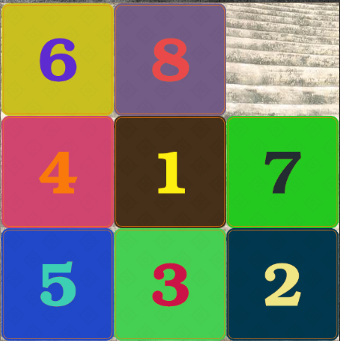
\includegraphics[width=0.5\linewidth]{puzzle8.png}
		\caption{8-Puzzle initial state}
	\end{figure}
2\end{frame}

\begin{frame}
	\begin{figure}
	\centering
		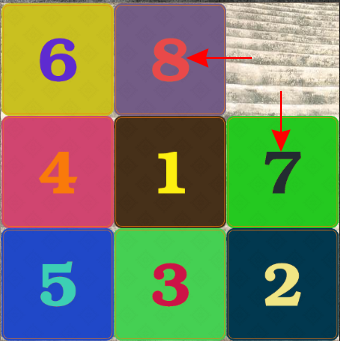
\includegraphics[width=0.5\linewidth]{puzzle8_arrows.png}
		\caption{8-Puzzle possible actions}
	\end{figure}
\end{frame}

\begin{frame}
	\begin{figure}
	\centering
		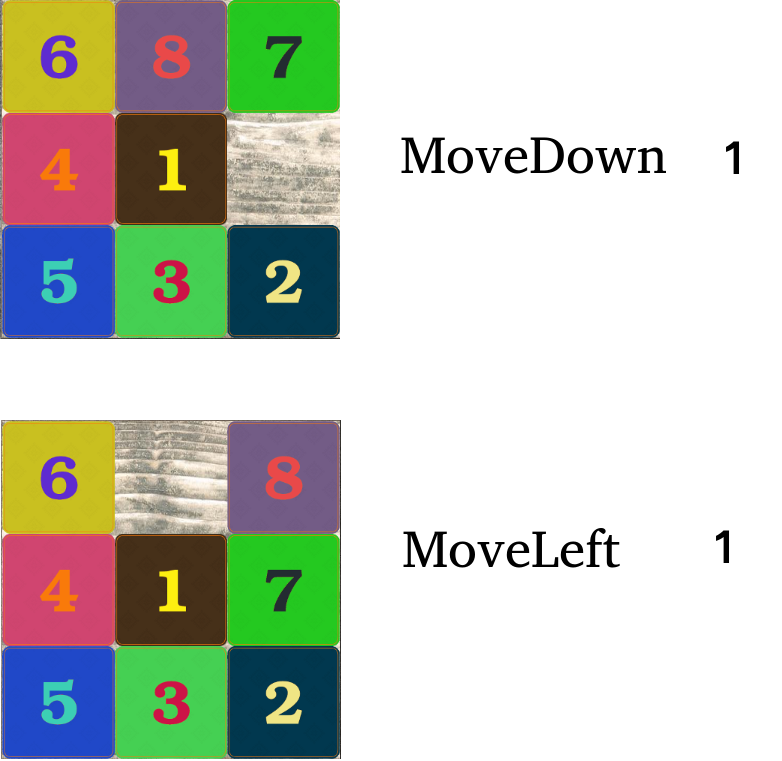
\includegraphics[width=0.5\linewidth]{puzzle8_successors.png}
		\caption{8-Puzzle list of successor triplets}
	\end{figure}
\end{frame}

\begin{frame}
	\begin{figure}
	\centering
		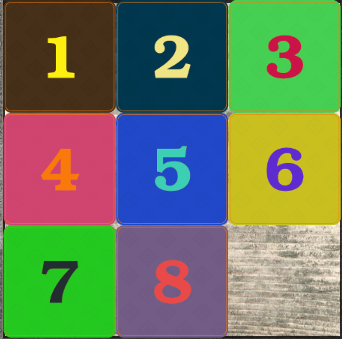
\includegraphics[width=0.5\linewidth]{puzzle8_goal.png}
		\caption{8-Puzzle goal state}
	\end{figure}
\end{frame}

\subsection{Pathfinding}

\begin{frame}
	\begin{figure}
	\centering
		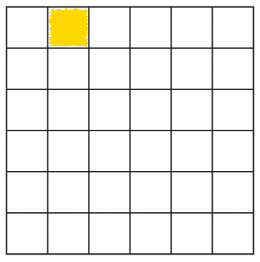
\includegraphics[width=0.5\linewidth]{pathfinding.png}
		\caption{Pathfinding initial state}
	\end{figure}
\end{frame}

\begin{frame}
	\begin{figure}
	\centering
		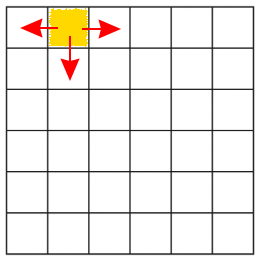
\includegraphics[width=0.5\linewidth]{pathfinding_arrows.png}
		\caption{Pathfinding possible actions}
	\end{figure}
\end{frame}

\begin{frame}
	\begin{figure}
	\centering
		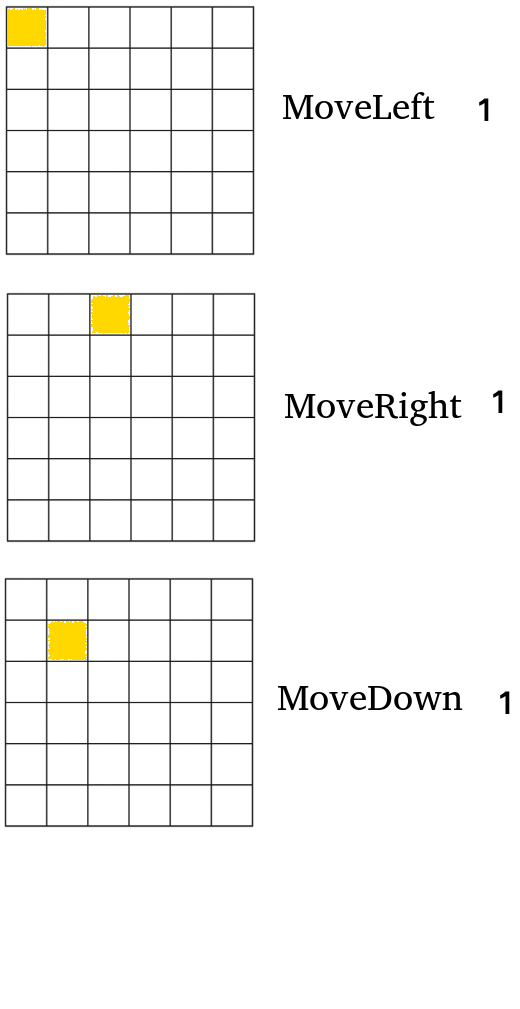
\includegraphics[width=0.3\linewidth]{pathfinding_successors.png}
		\caption{Pathfinding list of successor triplets}
	\end{figure}
\end{frame}

\begin{frame}{State space graph}
	\pause
	\begin{figure}
	\centering
		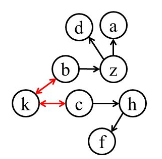
\includegraphics[width=0.6\linewidth]{state_space_graph.png}
		\caption{State space graph}
	\end{figure}
\end{frame}

\section{Search algorithm}

\subsection{Search tree}

\begin{frame}{Search tree}

	\begin{figure}
	\centering
		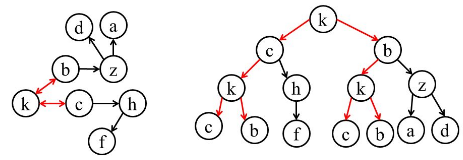
\includegraphics[width=\linewidth]{state_space_vs_search_tree.png}
		\caption{State space vs search tree}
	\end{figure}

\end{frame}

\begin{frame}{Nodes}

	\begin{itemize}
		\item Open nodes - known but unexplored
		\item Closed nodes - explored i.e. checked against goal state and their successors were queried
	\end{itemize}

\end{frame}

\subsection{General algorithm pseudocode}

\begin{frame}[fragile]{General algorithm pseudocode}
	\begin{lstlisting}
closedNodes = {}
openNodes = {}

openNodes.insert(getInitialState())
while openNodes not empty 
	node = openNodes.get()
	if isGoalState(node)
		return node
		
	if node in closedNodes
		continue
		
	for childNode in getSuccessors(node)
		if childNode not in closedNodes
			openNodes.insert(childNode)
	closedNodes.insert(node)
	\end{lstlisting}
\end{frame}

\section{Blind algorithms}

\begin{frame}{Working example}

	\begin{figure}
	\centering
		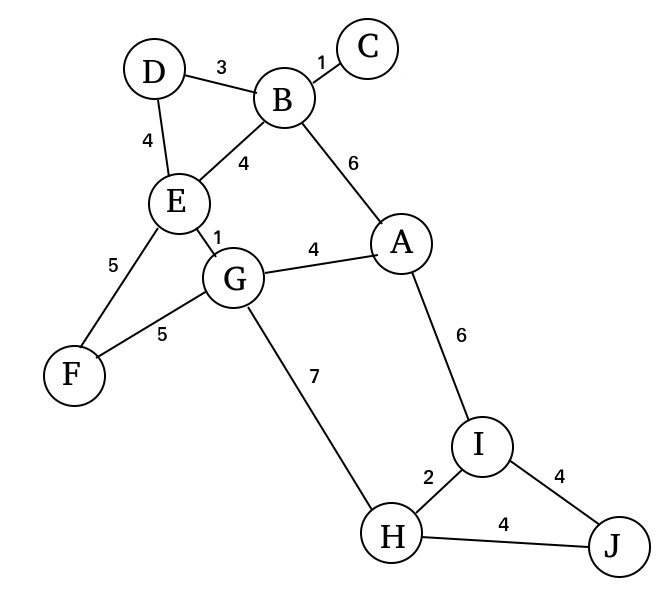
\includegraphics[width=0.8\linewidth]{example.jpg}
	\end{figure}

\end{frame}

\begin{frame}{Blind algorithms}

	\begin{columns}[T]
	
		\begin{column}{.48\textwidth}
			\begin{figure}
			\centering
				
\includegraphics[width=\linewidth]{spongebob_blind.jpg}
			\end{figure}
		\end{column}
		
		\begin{column}{.48\textwidth}
		
			\begin{itemize}
				\item no additional information about the problem
				\item needs to figure everything out on it's own
			\end{itemize}
		
		\end{column}
	
	\end{columns}

\end{frame}

\subsection{Breadth first search (BFS)}

\begin{frame}[fragile]{Breadth First Search (BFS)}
	\begin{lstlisting}
closedNodes = {}

# First In First Out
openNode = Queue()

openNodes.insert(getInitialState())
while openNodes not empty 
	node = openNodes.get()
	if isGoalState(node)
		return node
	if node in closedNodes
		continue				
	for childNode in getSuccessors(node)
		if childNode not in closedNodes
			openNodes.insert(childNode)
	closedNodes.insert(node)
	\end{lstlisting}
\end{frame}

\begin{frame}{Breadth First Search (BFS)}
	\begin{columns}[T]
		\begin{column}{.48\textwidth}
			\begin{figure}
			\centering
				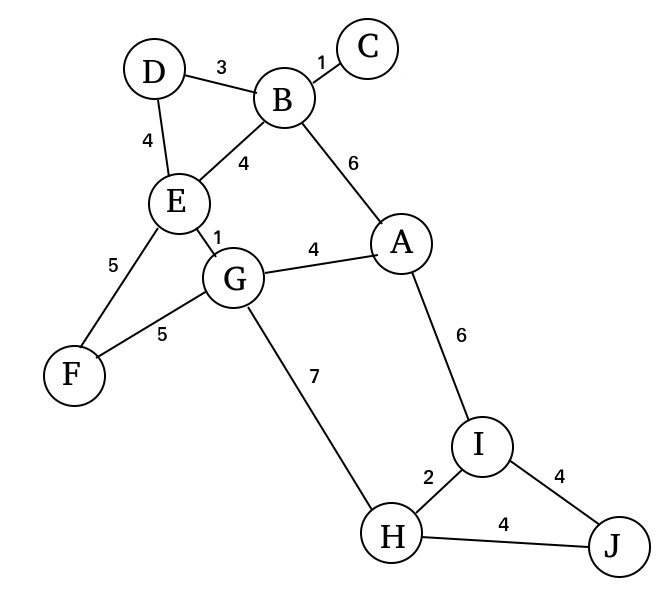
\includegraphics[width=1.3\linewidth]{example.jpg}
			\end{figure}
		\end{column}
		
		\begin{column}{.48\textwidth}
				\begin{itemize}
					\item Find a path from B to I
					\newline
					\only<1>{
						\item OPEN: {[ B ]}
						\newline
						\item CLOSED: \{\}
					}
					\only<2>{
						\item OPEN: {[ \textcolor{green}{C, D, E, A} ]}
						\newline
						\item CLOSED: \{ \textcolor{red}{B} \}					
					}
					\only<3>{
						\item OPEN: {[ D, E, A ]}
						\newline
						\item CLOSED: \{ B, \textcolor{red}{C} \}
					}
					\only<4>{
						\item OPEN: {[ E, A ]}
						\newline
						\item CLOSED: \{ B, C, \textcolor{red}{D} \}
					}
					\only<5>{
						\item OPEN: {[ A, \textcolor{green}{F, G} ]}
						\newline
						\item CLOSED: \{ B, C, D, \textcolor{red}{E} \}
					}
					\only<6>{
						\item OPEN: {[ F, G, \textcolor{green}{I} ]}
						\newline
						\item CLOSED: \{ B, C, D, E, \textcolor{red}{A} \}
					}
					\only<7>{
						\item OPEN: {[ G, I ]}
						\newline
						\item CLOSED: \{ B, C, D, E, A, \textcolor{red}{F} \}
					}
					\only<8>{
						\item OPEN: {[ I, \textcolor{green}{H} ]}
						\newline
						\item CLOSED: \{ B, C, D, E, A, F, \textcolor{red}{G} \}
					}
					\only<9>{
						\item Reached goal I
					}

				\end{itemize}
		\end{column}
	\end{columns}
\end{frame}

\begin{frame}{Breadth First Search (BFS)}
	\begin{figure}
		\centering
		\only<1>{
			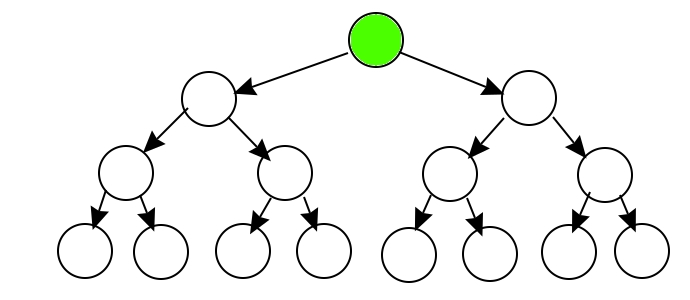
\includegraphics[width=\linewidth]{search_tree_example.jpg}
		}
		\only<2>{
			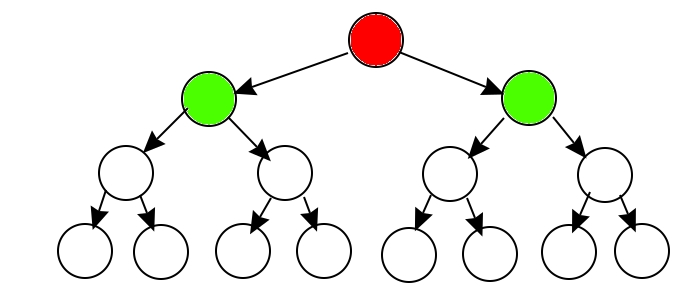
\includegraphics[width=\linewidth]{search_tree_bfs_1.jpg}
		}
		\only<3>{
			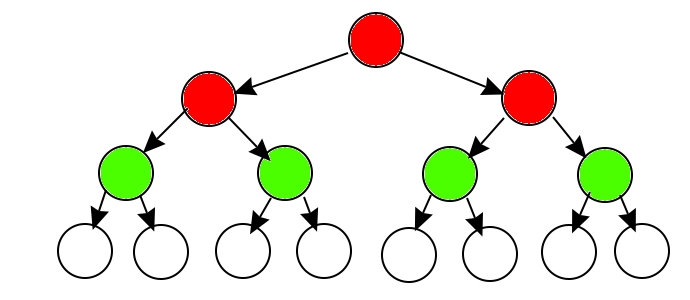
\includegraphics[width=\linewidth]{search_tree_bfs_2.jpg}
		}
		\only<4>{
			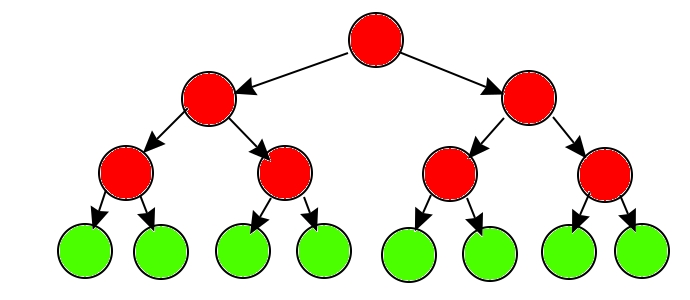
\includegraphics[width=\linewidth]{search_tree_bfs_3.jpg}
		}
	\end{figure}
\end{frame}

\subsection{Depth first search (DFS)}

\begin{frame}[fragile]{Depth First Search (DFS)}
	\begin{lstlisting}
closedNodes = {}

# Last In First Out
openNode = Stack()

openNodes.insert(getInitialState())
while openNodes not empty 
	node = openNodes.get()
	if isGoalState(node)
		return node
	if node in closedNodes
		continue				
	for childNode in getSuccessors(node)
		if childNode not in closedNodes
			openNodes.insert(childNode)
	closedNodes.insert(node)
	\end{lstlisting}
\end{frame}

\begin{frame}{Depth First Search (DFS)}
	\begin{columns}[T]
		\begin{column}{.48\textwidth}
			\begin{figure}
			\centering
				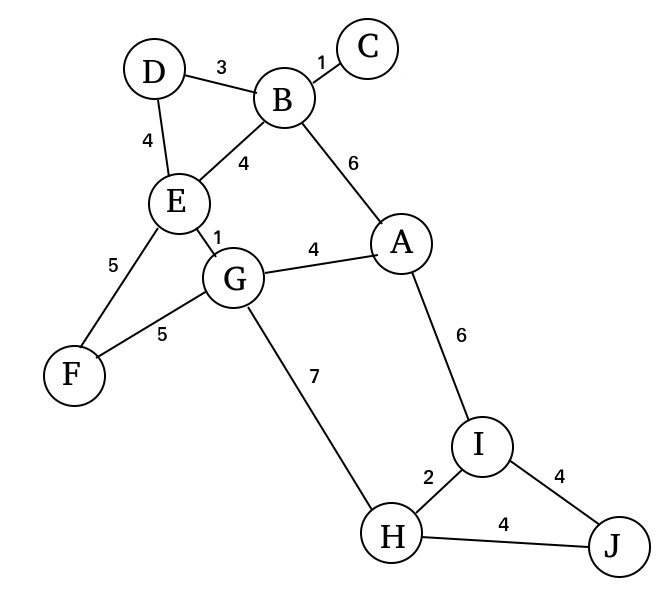
\includegraphics[width=1.3\linewidth]{example.jpg}
			\end{figure}
		\end{column}
		
		\begin{column}{.48\textwidth}
				\begin{itemize}
					\item Find a path from B to I
					\newline
					\only<1>{
						\item OPEN: {[ B ]}
						\newline
						\item CLOSED: \{\}
					}
					\only<2>{
						\item OPEN: {[ \textcolor{green}{C, D, E, A} ]}
						\newline
						\item CLOSED: \{ \textcolor{red}{B} \}					
					}
					\only<3>{
						\item OPEN: {[ D, E, A ]}
						\newline
						\item CLOSED: \{ B, \textcolor{red}{C} \}
					}
					\only<4>{
						\item OPEN: {[ E, A ]}
						\newline
						\item CLOSED: \{ B, C, \textcolor{red}{D} \}
					}
					\only<5>{
						\item OPEN: {[ \textcolor{green}{F, G}, A ]}
						\newline
						\item CLOSED: \{ B, C, D, \textcolor{red}{E} \}
					}
					\only<6>{
						\item OPEN: {[ G, A ]}
						\newline
						\item CLOSED: \{ B, C, D, E, \textcolor{red}{F} \}
					}
					\only<7>{
						\item OPEN: {[ \textcolor{green}{H}, A ]}
						\newline
						\item CLOSED: \{ B, C, D, E, F, \textcolor{red}{G} \}
					}
					\only<8>{
						\item OPEN: {[ \textcolor{green}{I, J}, A ]}
						\newline
						\item CLOSED: \{ B, C, D, E, F, G, \textcolor{red}{H} \}
					}
					\only<9>{
						\item Reached goal I
					}

				\end{itemize}
		\end{column}
	\end{columns}
\end{frame}

\begin{frame}{Depth First Search (DFS)}
	\begin{figure}
		\centering
		\only<1>{
			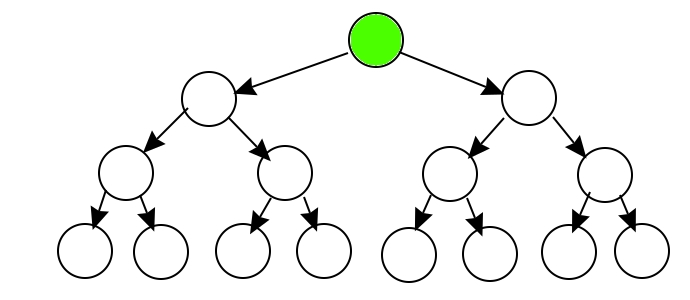
\includegraphics[width=\linewidth]{search_tree_example.jpg}
		}
		\only<2>{
			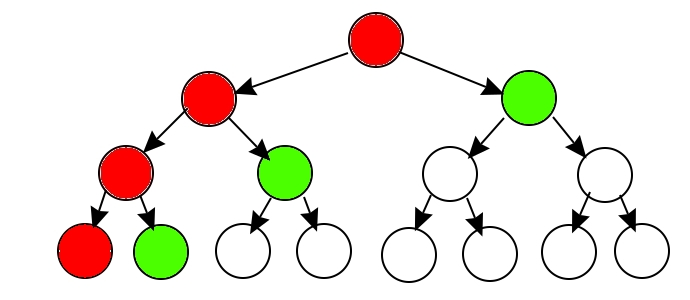
\includegraphics[width=\linewidth]{search_tree_dfs_1.jpg}
		}
		\only<3>{
			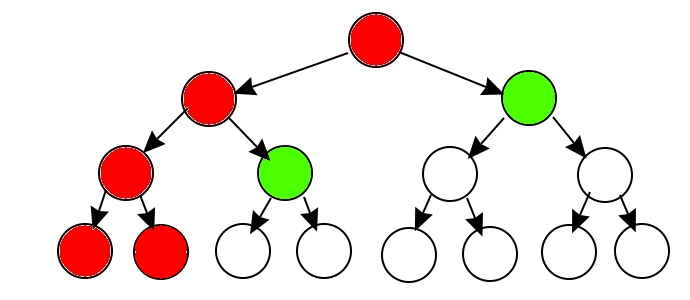
\includegraphics[width=\linewidth]{search_tree_dfs_2.jpg}
		}
		\only<4>{
			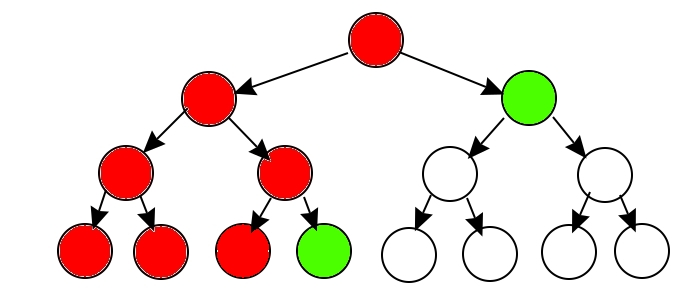
\includegraphics[width=\linewidth]{search_tree_dfs_3.jpg}
		}
		\only<5>{
			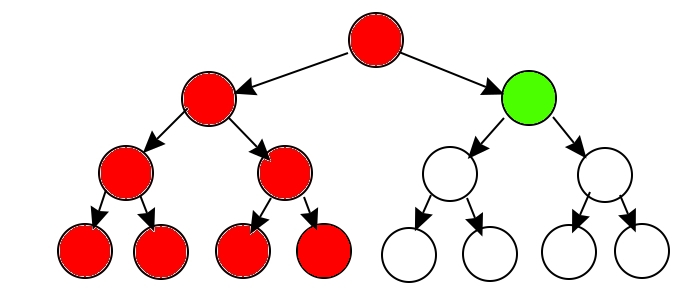
\includegraphics[width=\linewidth]{search_tree_dfs_4.jpg}
		}
		\only<6>{
			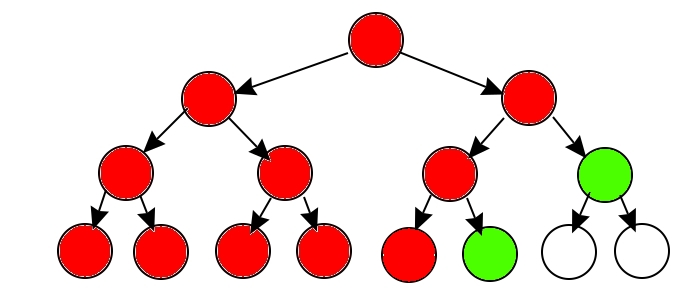
\includegraphics[width=\linewidth]{search_tree_dfs_5.jpg}
		}
	\end{figure}
\end{frame}

\subsection{Uniform cost search (UCS)}


% TO-FUCKING-DO
\begin{frame}[fragile]{Uniform Cost Search (UCS)}
	\begin{lstlisting}
closedNodes = {}

# First In First Out
openNode = Queue()

openNodes.insert(getInitialState())
while openNodes not empty 
	node = openNodes.get()
	if isGoalState(node)
		return node
	if node in closedNodes
		continue				
	for childNode in getSuccessors(node)
		if childNode not in closedNodes
			openNodes.insert(childNode)
	closedNodes.insert(node)
	\end{lstlisting}
\end{frame}

\begin{frame}{Breadth First Search (BFS)}
	\begin{columns}[T]
		\begin{column}{.48\textwidth}
			\begin{figure}
			\centering
				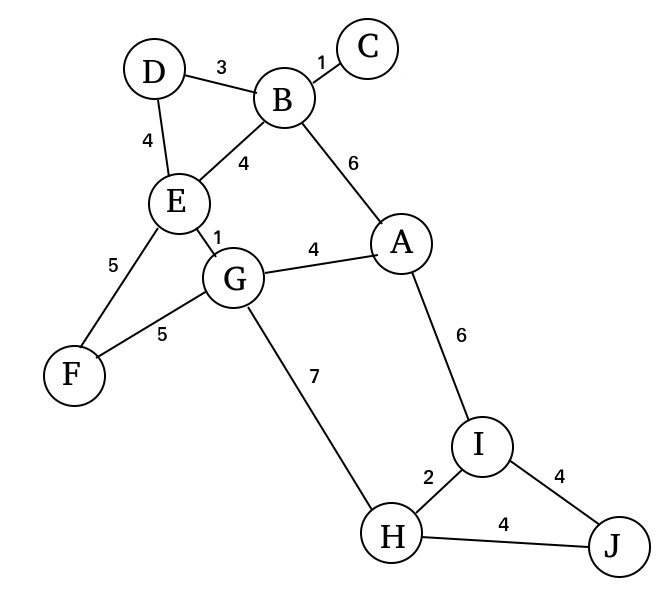
\includegraphics[width=1.3\linewidth]{example.jpg}
			\end{figure}
		\end{column}
		
		\begin{column}{.48\textwidth}
				\begin{itemize}
					\item Find a path from B to I
					\newline
					\only<1>{
						\item OPEN: {[ B ]}
						\newline
						\item CLOSED: \{\}
					}
					\only<2>{
						\item OPEN: {[ \textcolor{green}{C, D, E, A} ]}
						\newline
						\item CLOSED: \{ \textcolor{red}{B} \}					
					}
					\only<3>{
						\item OPEN: {[ D, E, A ]}
						\newline
						\item CLOSED: \{ B, \textcolor{red}{C} \}
					}
					\only<4>{
						\item OPEN: {[ E, A ]}
						\newline
						\item CLOSED: \{ B, C, \textcolor{red}{D} \}
					}
					\only<5>{
						\item OPEN: {[ A, \textcolor{green}{F, G} ]}
						\newline
						\item CLOSED: \{ B, C, D, \textcolor{red}{E} \}
					}
					\only<6>{
						\item OPEN: {[ F, G, \textcolor{green}{I} ]}
						\newline
						\item CLOSED: \{ B, C, D, E, \textcolor{red}{A} \}
					}
					\only<7>{
						\item OPEN: {[ G, I ]}
						\newline
						\item CLOSED: \{ B, C, D, E, A, \textcolor{red}{F} \}
					}
					\only<8>{
						\item OPEN: {[ I, \textcolor{green}{H} ]}
						\newline
						\item CLOSED: \{ B, C, D, E, A, F, \textcolor{red}{G} \}
					}
					\only<9>{
						\item Reached goal I
					}

				\end{itemize}
		\end{column}
	\end{columns}
\end{frame}

\section{Heuristic algorithms}

\subsection{Heuristics}

\subsection{Greedy search}

\subsection{A* search}


\section{Unity engine - NavMesh}


\end{document}